\RequirePackage{pgfornament,tkzexample,tikzrput}  



\documentclass[a5paper,oneside]{amsart}
\usepackage[scale={.9,.9}]{geometry}
\usepackage{mathrsfs}
\usepackage[utf8]{inputenc}
\usepackage{amsthm}
\usepackage{amsmath}
\usepackage{bbold}
\usepackage{dsfont}
\usepackage{chngcntr}



\newtheoremstyle{dotless}{}{}{\itshape}{}{\bfseries}{}{ }{}
\theoremstyle{dotless}
\renewenvironment{proof}{{\bfseries Demostración:}}



\newtheorem{teorema}{\;\;Teorema}[section]
\newtheorem{problema}[teorema]{\;\;Problema}
\newtheorem{definicion}[teorema]{\;\;Definición}
\newtheorem*{categoria}{Categorías:}
\newtheorem*{remark}{Remark}
\setcounter{secnumdepth}{3}
\setcounter{tocdepth}{3}


%\setlength{\textwidth}{17.2cm} % was 18.2
%\setlength{\textheight}{23cm} % was 23
%\setlength{\topmargin}{-1cm} % was 0
%\setlength{\oddsidemargin}{-0.6cm}
%\setlength{\evensidemargin}{-0.6cm}

%\setlength{\textwidth}{18.9cm} % was 18.2
%\setlength{\textheight}{26.73cm} % was 23
%\setlength{\topmargin}{1cm} % was 0
%\setlength{\oddsidemargin}{0cm} %
%\setlength{\evensidemargin}{.8cm}
%% Arreglar pues ahora utilizas papel A4.

%Operadores

\DeclareMathOperator{\ivp}{IVP} %
\DeclareMathOperator{\sgn}{sgn} %
\DeclareMathOperator{\md}{mod}
\DeclareMathOperator{\ima}{Im}%
\DeclareMathOperator{\id}{Id} %
\DeclareMathOperator{\homo}{Hom} %
\DeclareMathOperator{\inter}{Int}
\DeclareMathOperator*{\Lim}{lim}
\DeclareMathOperator*{\Limsup}{lim\ sup}
\DeclareMathOperator*{\Liminf}{lim\ inf}
\DeclareMathOperator*{\Min}{m\text{\ii}n}
\DeclareMathOperator{\Aff}{Aff}
\DeclareMathOperator{\Affb}{\overline{\Aff}}
\DeclareMathOperator{\sdfd}{dfd}
\DeclareMathOperator{\scdfd}{dfd}
\DeclareMathOperator{\Beta}{B}
\DeclareMathOperator{\pd}{PD}
\DeclareMathOperator{\supp}{supp}
\DeclareMathOperator{\diam}{diam}
\newcommand{\ind}{\operatornamewithlimits{\perp}}
\DeclareMathOperator{\av}{Abs}
\DeclareMathOperator{\cb}{CB}
\DeclareMathOperator{\cbi}{CBI}
\DeclareMathOperator{\gwi}{GWI}
\DeclareMathOperator{\gw}{GW}
\newcommand{\rtree}{$\re$\nbd tree}
\newcommand{\leb}{\text{Leb}}
%Notaci?n



%Delimitadores
\newcommand{\ceil}[1]{\ensuremath{\lceil #1 \rceil}}
%\renewcommand{\floor}[1]{\ensuremath{\lfloor #1 \rfloor}}

%Formato
\newcommand{\defin}[1]{{\bf #1}}
\newcommand{\mc}[1]{\ensuremath{\mathscr{#1}}}
\newcommand{\bb}[1]{\mathbb{#1}}


%Notation

\newcommand{\card}[1]{\ensuremath{\left| #1 \right|}}
\newcommand{\lccb}{LCCB}
\newcommand{\pss}{S}
\newcommand{\compact}{K}
\newcommand{\psm}{\rho}
\newcommand{\ps}{\paren{\pss,\psm}}
\newcommand{\pse}{x}
\newcommand{\psep}{y}
\newcommand{\psepp}{z}
\newcommand{\saps}{\B_{\pss}}
\newcommand{\bre}{\B_{\re}}
\newcommand{\sko}{D}
\newcommand{\trees}{T}
\newcommand{\C}{C}
\newcommand{\refm}{\mu}
\newcommand{\den}{p}
\newcommand{\psd}[1]{\mc{P}_{#1}}
\newcommand{\s}{\ensuremath{\sigma}}
\newcommand{\bden}{M}
\newcommand{\hh}[1]{{\bf H#1}}
\newcommand{\ball}[2]{\imf{B_{#1}}{#2}}
\newcommand{\mmc}[1]{\imf{\tilde\omega}{#1}}
\newcommand{\rg}[1]{\ensuremath{\imf{\mathbb{G}}{#1}}}




\newcommand{\dfd}{\ensuremath{\stackrel{\sdfd}{=}}}
\newcommand{\deq}{\ensuremath{\stackrel{d}{=}}}

\newcommand{\ley}[2]{\ensuremath{\imf{\mc{L}^{#2}}{#1}}}
\newcommand{\leyc}[3]{\ensuremath{\imf{\mc{L}^{#3}}{#1\left|#2\right.}}}
\newcommand{\cond}[2]{\left.\vphantom{#2}#1\ \right| #2}

\newcommand{\e}{\ensuremath{\mathbf{e}}}
\newcommand{\esf}{\ensuremath{\mc{S}^{\downarrow}}}
%\newcommand{\ps}[1]{\mathscr{P}\paren{#1}}
\newcommand{\fun}[3]{\ensuremath{#1:#2\to #3}}
\newcommand{\fund}[3]{\ensuremath{#1:#2\mapsto #3}}
\newcommand{\set}[1]{\ensuremath{\left\{ #1\right\} }}
\newcommand{\sets}[1]{\ensuremath{{\mathbf #1}}}
\newcommand{\paren}[1]{\ensuremath{\left( #1\right) }}
\newcommand{\bra}[1]{\ensuremath{\left[ #1\right] }}
\newcommand{\seq}[1]{\ensuremath{ #1 _1,\ldots ,#1 _n }}
\newcommand{\sm}[3]{\left[ #1\right]_{#2}^{#3}}
\newcommand{\cde}{\Rightarrow}
\newcommand{\cdfd}{\ensuremath{\stackrel{\scdfd}{\cde}}}
\newcommand{\convo}[2]{\ensuremath{#2^{\!* #1}}}

\newcommand{\tl}[1]{\ensuremath{\hat{#1}}}

\newcommand{\matt}[3]{#1_{#2\, #3}}
\newcommand{\sip}{\bb{P}}
\newcommand{\jump}[2]{\ensuremath{\Delta #1_{#2}}}
\newcommand{\cadlag}{c\`adl\`ag}
\newcommand{\se}{\ensuremath{\bb{E}}}
\newcommand{\ssa}{\ensuremath{\mathscr{F}}}
\newcommand{\si}{{\ensuremath{\bf{1}}}}
\newcommand{\sbr}{\ensuremath{\mc{B}_{\re}}}
%\newcommand{\siind}{\ensuremath{\perp}}
\newcommand{\sigam}{\ensuremath{\Gamma}}
\newcommand{\smc}{\ensuremath{m}}
\newcommand{\sfleche}{S^{\downarrow}_f}

\newcommand{\gafun}[1]{\sigam \paren{#1}}
\newcommand{\poi}[1]{\ensuremath{\mc{P}\!_{#1}}}
\newcommand{\ber}[1]{\ensuremath{\mc{B}\!_{#1}}}
\newcommand{\fcpoi}[1]{\ensuremath{\hat{\mc{P}}\!_{#1}}}
%\newcommand{\ind}{\siind}
\newcommand{\condind}[3]{\ensuremath{#1\ind_{#3}#2}}
\newcommand{\sig}[1]{$\sigma$-\nobreakdash #1}
\newcommand{\sa}{\ensuremath{\sigma}\nbd field}
\newcommand{\realtree}{\ensuremath{\re}\nbd tree}
\newcommand{\eps}{\ensuremath{ \varepsilon}}
\newcommand{\na}{\ensuremath{\mathbb{N}}}
\newcommand{\en}{\ensuremath{\mathbb{Z}_+}}
\newcommand{\eti}{\ensuremath{\mc{U}}}
\newcommand{\etic}{\ensuremath{\mathbb{U}}}
\newcommand{\z}{\ensuremath{\mathbb{Z}}}
\newcommand{\re}{\ensuremath{\mathbb{R}}}
\newcommand{\ra}{\ensuremath{\mathbb{Q}}}
\newcommand{\com}{\ensuremath{\mathbb{C}}}
\newcommand{\con}[1]{\ensuremath{\overline{#1}}}
\newcommand{\proba}[1]{\ensuremath{\sip\! \left( #1 \right)}}
\newcommand{\probas}[2]{\ensuremath{#1\! \left( #2 \right)}}
\newcommand{\probac}[2]{\ensuremath{\sip\! \left( #1 \, | #2 \right)}}
\newcommand{\esp}[1]{\ensuremath{\se\! \left( #1 \right)}}
%\newcommand{\espc}[2]{\ensuremath{\se\! \left( #1 | #2 \right)}}
\newcommand{\espc}[2]{\ensuremath{\imf{\se}{\cond{#1}{#2}}}}
\newcommand{\var}[1]{\ensuremath{\text{Var}\! \left( #1 \right)}}
\newcommand{\cov}[1]{\ensuremath{Cov\! \left( #1 \right)}}
\newcommand{\abs}[1]{\hspace{.25mm}\left|#1\right|\hspace{.25mm}}
\newcommand{\ila}[2]{\ensuremath{\int #1\, d#2}}
\newcommand{\ilas}[3]{\ensuremath{\int_{#1} #2\, d#3}}
\newcommand{\il}[3]{\ensuremath{\int #1\, \imf{#2}{d#3}}}
\newcommand{\is}[4]{\ensuremath{\int_{#1} #2\, \imf{#3}{d#4}}}
\newcommand{\lp}[2]{\ensuremath{\mc{L}_#1\!\paren{#2} }}
\newcommand{\lpc}[4]{\ensuremath{\mc{L}_#1\!\paren{ #2 , #3 , #4 }}}
\newcommand{\ip}[1]{\ensuremath{\int #1\, d\sip }}
\newcommand{\ips}[2]{\ensuremath{\int_{#1} #2\, d\sip}}
\newcommand{\uF}{\ssa^u}
\newcommand{\G}{\ensuremath{\mc{G}}}
\newcommand{\h}{\ensuremath{\mc{H}}}
\newcommand{\B}{\ensuremath{\mc{B}}}
\newcommand{\f}[1]{\ssa_{#1}}
\newcommand{\fx}[2]{\ssa_{#1}^{#2}}
\newcommand{\indi}[1]{\si_{#1}}
\newcommand{\imi}[2]{#2^{-1}\!\paren{#1}}
\newcommand{\ooo}{\ensuremath{ \omega  } }
\newcommand{\oo}{\ensuremath{ \Omega  } }
\newcommand{\p}{\ensuremath{ \sip  } }
\newcommand{\q}{\ensuremath{ \bb{Q}  } }
\newcommand{\ofp}{\ensuremath{ \paren{ \Omega ,\F ,\p } } }
\newcommand{\med}[2]{\ensuremath{\paren{#1}{#2}}-medible}
\newcommand{\vat}{\ensuremath{\fun{X}{\oo}{\re}}\ }
\newcommand{\pix}[1]{\ensuremath{\sip}_{\! #1}}
\newcommand{\px}[2]{\ensuremath{\sip_{\! #1}\!\paren{#2}}}
\newcommand{\pxc}[3]{\ensuremath{\sip_{\! #1}\!\left( #2 | #3 \right)}  }
\newcommand{\br}{\sbr}
\newcommand{\sag}[1]{\sigma\!\paren{#1}}
\newcommand{\cs}[1]{\ensuremath{#1}-p.s.}
\newcommand{\ore}{ \ensuremath{\overline{\re}}}
\newcommand{\fungen}[1]{\ensuremath{\varphi_{#1}}}%Comando para la notaci�n de funci�n generadora.
\newcommand{\cbin}[2]{\ensuremath{\paren{\begin{array}{c}#1\\#2\end{array}}}}
\newcommand{\fa}[2]{\ensuremath{{#1}^{\paren{#2}}}}
\newcommand{\dnor}[2]{\ensuremath{N(#1,#2)}}
\newcommand{\mb}{movimiento browniano}
\newcommand{\moc}[3]{\smc^{#3}(#1,#2)}
\newcommand{\clo}[1]{\ensuremath{\overline{#1}}}
\newcommand{\inte}[1]{\ensuremath{\inter #1}}
\newcommand{\fro}[1]{\ensuremath{\partial\paren{ #1}}}
\newcommand{\cd}[2]{\ensuremath{#1\stackrel{\mc{D}}{\to}#2}}
\newcommand{\pr}[3]{\ensuremath{#1_{#2}\!\paren{#3}}}
\newcommand{\oi}[1]{\ensuremath{\mc{O}\paren{#1}}}
\newcommand{\mw}{\ensuremath{\mathbb{P}}}
\newcommand{\me}{\ensuremath{\pi}}


\newcommand{\nbd}{\nobreakdash -}
\newcommand{\ii}{\'{\i}}
\newcommand{\n}{\~n}
\newcommand{\imf}[2]{\ensuremath{#1\!\paren{#2}}}
\newcommand{\floor}[1]{\ensuremath{\lfloor #1\rfloor}}
\newcommand{\proint}[2]{\ensuremath{\langle #1,#2\rangle}}
\newcommand{\vp}{\ensuremath{\varphi}}
\newcommand{\noru}[1]{\ensuremath{\|#1\|}}
\newcommand{\gen}[1]{\ensuremath{|#1 |}}
\newcommand{\vc}[1]{\ensuremath{\langle #1\rangle}}
\newcommand{\pc}[2]{\ensuremath{\langle#1,#2\rangle}}
\newcommand{\vcd}[1]{\ensuremath{\left[#1\right]}}

\newcommand{\sml}{\ensuremath{\nu}}
\newcommand{\ml}[1]{\ensuremath{\imf{\sml}{#1}}}
\newcommand{\va}[2]{\ensuremath{\imf{V_{#1}}{#2}}}
\newcommand{\clase}[1]{\ensuremath{\mc{C}^{#1}}}
\newcommand{\marte}[2]{\ensuremath{\imf{\mc{E}^{#2}}{#1}}}

\newcommand{\dencero}[1]{\ensuremath{\left. \frac{\partial }{\partial #1}\right|_{#1=0} }}
%\newcommand{\premin}[1]{\ensuremath{\stackrel{\leftarrow}{#1}}}
%\newcommand{\postmin}[1]{\ensuremath{\stackrel{\rightarrow}{#1}}}
\newcommand{\premin}[1]{\ensuremath{{#1}^{\leftarrow}}}
\newcommand{\postmin}[1]{\ensuremath{{#1}^{\rightarrow}}}



%Ambientes (Environments)

\newenvironment{esn}{\begin{equation*}}{\end{equation*}}
\newenvironment{ecn}{\begin{equation}}{\end{equation}}
\newenvironment{listeo}{\begin{list}{\alph{enumi})}{\usecounter{enumi}}}{\end{list}}
\newenvironment{numerai}{\begin{list}{\roman{enumi})}{\usecounter{enumi}}}{\end{list}}
\newcommand{\N}{\mathbb{N}}
\newcommand{\R}{\mathbb{R}}
\newcommand{\E}{\mathbb{E}}

\newcommand{\F}{\mathscr{F}}

\newcommand{\indic}{\mathds{1}}

\newcommand{\textme}[1]{\;\text{#1}\;}
\newcommand{\nqed}{
	\null
	\null
	\null
	\null	
	\center{
		\textbf{---------------------------------------------------------------------------------------}
	}
	\newpage
}


\renewcommand{\nqed}
{		
		\null
		\null
		\null
		\null
		\begin{tikzpicture}
			\node (A) at (0,0) {};
			\node (B) at (3,0) {};
			\node (C) at (6,0) {};
			\path (A.center) to [ornament=86,at=0] (B.center);
			\path (A.center) to [ornament=85,at=0.50] (B.center);
			\path (A.center) to [ornament=88,at=0.75] (C.center);
    		\path (B.center) to [ornament=85,at=1.50] (C.center);
			\path (B.center) to [ornament=86,at=2] (C.center);
		\end{tikzpicture}\\
		\newpage
}




\title[Problemas de Procesos I]{Problemas de Procesos Estocásticos I\\ Semestre 2013-II\\ Posgrado en Ciencias Matemáticas\\ Universidad Nacional Autónoma de México}

\usepackage[colorlinks,citecolor=blue,urlcolor=blue]{hyperref}

\begin{document}
	\maketitle
	\section{Tarea 1}
	\nqed
		\subsection{problema1.1}
		\begin{problema}
	Sea $\left({X_n}_{n\in\mathbb{N}}\right)$ un proceso estocástico con valores reales y $A\subset \mathbb{R}$ un boreliano. 
	Pruebe que si
	\begin{align}
		T_0=0\quad\text{y}\quad T_{n+1}=\min\{k>T_n: X_k\in A \subset \mathbb{R}\}
	\end{align}
	entonces $T_n$ es un tiempo de paro para toda $n$ y $T_n\to \infty$ puntualmente conforme $n\to\infty$. 

	\begin{categoria} 
		Tiempos de paro.
	\end{categoria}
\end{problema}
		
\begin{proof}
\\

	Sea $(\mathscr{F}_n = \sigma(  X_0, X_1, \dots, X_n ))_{ n \in \mathbb{N}}$ una filtración.
\\

	Veamos que $T_0$ es tiempo de paro. $\{T_0 = 0\} = \Omega \in \mathscr{F}_n$ y 
	$\{T_0 = c\} = \emptyset \in \mathscr{F}_n$ para $c \not= 0 \in \mathbb{N}$. Recordemos que:		
	\begin{align}\label{problema_1_1:equivalencia_varable_aleatoria}
		\{T_0 = n\} \in \mathscr{F}_n \; \forall n \in \mathbb{N} \iff 
		\{T_0 \leq n\} \in \mathscr{F}_n \; \forall n \in \mathbb{N}.
	\end{align}
	Y por lo tanto $T_0$ es variable aleatoria sobre la sigma álgebra $\sigma(\cup_{n \in \mathbb{N}} 
	\mathscr{F}_n)$.

	Para $n=1$, veamos que:
 
	\begin{align}
			\{T_1 = 1\}     &= \{ X_1 \in A \}	\in \mathscr{F}_1 
	\end{align}
	
	\begin{align}
			\{T_1 = 2\} 	&= 	\{ X_1 \not\in A, X_2 \in A \} \\
							&= 	\{ X_1 \not\in A \} \cap \{X_2 \in A \} \in \mathscr{F}_2	
	\end{align}
	
	\begin{align}
			\{T_1 = 3\} 	&=	\{ X_1 \not\in A, X_2 \not\in A,  X_3 \in A \} \\ 
							&= 	\{ X_1 \not\in A \} \cap \{ X_2 \not\in A \} \cap \{X_3 \in A \} \in \mathscr{F}_3
	\end{align}
	
	\begin{align*}
		\vdots
	\end{align*}
	
	\begin{align}
			\{T_1 = n\} 	&=	\{ X_1 \not\in A, X_2 \not\in A, \dots, X_{n-1} \not\in A, X_n \in A \} \\
							&= 	\bigcap_{i=1}^{i=n-1} \{ X_i \not\in A \} \cap \{X_n \in A \} \in \mathscr{F}_n
	\end{align} 
 
	Por hipótesis de inducción supongamos que $\{T_k = n\} \in \mathscr{F}_n$ para cierta $k>1$ 
	y para toda $n \in \mathbb{N}$ . \\

	Para demostrar la primera parte del ejercicio, basta probar que $\{T_{k+1} = n\} \in \mathscr{F}_n$ para 
	toda $n \in \mathbb{N}$. Pues por lo dicho en (\ref{problema_1_1:equivalencia_varable_aleatoria}) resultarían ser 
	variables aleatorias en $\sigma(\cup_{n \in \mathbb{N}} \mathscr{F}_n)$.
	\\
	
	Dado que 
	\begin{align}\label{problema_1_1:T_n->infty}
		0=T_0<T_1<T_2<\dots<T_k
	\end{align}  
	tenemos que $\{ T_k = n\} = \emptyset \in \mathscr{F}_l$ para $n < k$. 
	
	Ahora, sea $n \geq k$
	
	\begin{align}\label{problema_1_1:T_k+1}
		\{ T_{k+1} = n\} = 
		\left( \bigcup_{i < n } \{T_k = i \} \right) 
		\cap 
		\left( \bigcap_{i < n} \{ X_i \not\in A \} \right)
		\cap
		\{ X_n \in A\}
	\end{align}
	
	
	Donde 
	\begin{itemize}
		\item	 $\{ T_k = i\} \in \mathscr{F}_n \; \forall i < n \in \mathbb{N} \; $ (Por hipótesis de inducción).	
		\item	 $\{ X_i \not \in A\} \in \mathscr{F}_n \; \forall i < n \in \mathbb{N} \;$ (Por ser $\mathscr{F}$ filtración).
		\item $\{ X_n \in A\} \in \mathscr{F}_n$ (Por ser $X_n$ variable aleatoria en $\mathscr{F}_n$)	
	\end{itemize}
	
	Y por lo tanto, (\ref{problema_1_1:T_k+1}) pertenece a $\mathscr{F}_n$. Con lo que termina la demostración de la primera parte del ejercicio.\\
	
	Ahora, de (\ref{problema_1_1:T_n->infty}) se sigue inmediatamente que que $T_n \rightarrow \infty$.
\end{proof}
		
		\subsection{problema1.2}
		\begin{problema}
		Suponga que \(T\) es un tiempo de paro tal que para algún 
		\(N\in\mathbb{N}\) y \(\varepsilon>0\) se tiene que para toda \(n\in\mathbb{N}\):
		\begin{equation}\label{problema1_2:hipotesis_del_problema}
		\mathbb{P} (T \leq N + n | F_n) > \varepsilon \text{ casi seguramente}
		\end{equation}
		Al verificar la desomposici\'on
		\begin{equation}\label{problema1_2:sugerencia_del_problema}
			\mathbb{P} (T>kN)= \mathbb{P} (T>kN,T>(k-1)N)
		\end{equation}
		pruebe por inducci\'on que para cada \(k=1,2,\ldots\):
		\begin{align}
			\mw(T>kN)\leq (1-\varepsilon)^k.
		\end{align}
		Pruebe que \( \mathbb{E}(T)<\infty \). 
	\begin{categoria} Tiempos de paro.\end{categoria}
\end{problema}

\begin{proof}
	Tenemos que: 
	
	\begin{align}
		(T>kN \Rightarrow T>(k-1)N 	&\Rightarrow (T>kN) \subset (T>(k-1)N) \\ 
									&\Rightarrow (T>kN) \cap (T>(k-1)N) = (T>kN) \\ 
									&\Rightarrow \mw(T>kN, T>(k-1)N) = \mw(T>kN)	
	\end{align}
		
	\textbf{Base de inducción.} $k=1$. Usando (\ref{problema1_2:hipotesis_del_problema}), con $n=0$ 
	\begin{align}
		\mw(T\leq 1N | \F_0) > \epsilon\Rightarrow
		\mw(T>N| \F_0) < 1 - \epsilon
	\end{align}
	Sustituyendo por la definición de probabilidad condicional tenemos:
		\begin{align}
			\E(\indic_{T>N} | \F_0)	&= \mw(T>N| \F_0) 
									&< 1 - \epsilon
		\end{align}
	Aplicando esperanza en ambos lados tenemos:
		\begin{align} 
			\mw(T>N) 	&= 	\E(\E(\indic_{T>N} | \F_0)) 
						&< 	\E(1 - \epsilon) 
						&= 1 - \epsilon.
		\end{align}
	
	\textbf{Hipótesis de induccion.} Supongamos que $\mw(T>k_0N)\leq(1 - \epsilon)^{k_0}$ para algún $k_0 \geq 1$.
	
	\textbf{Paso inductivo.} 
	Utilizando (\ref{problema1_2:sugerencia_del_problema}) tenemos que
		\begin{align}
			\mw(T>(k_0+1)N) = \mw(T>(k_0+1)N, T>k_0N) = \E(\indic_{T>(k_0+1)N} \cdot \indic_{T>k_0N}).
		\end{align}
	Ahora, dado que $T>k_0N$ es un conjunto $\F_{k_0N}$-medible tenemos:
	\begin{align} 
		\E(\indic_{T>(k_0+1)N} \cdot \indic_{T>k_0N}) 	&=		\E\left(\E\left(\indic_{T>(k_0+1)N} \cdot \indic_{T>k_0N} | \F_{k_0N}\right)\right) \\ 
														&=		\E\left(\indic_{T>k_0N} \E\left(\indic_{T>(k_0+1)N}|\F_{k_0N}\right)\right) \label{problema1_2:resultado_preliminar}
	\end{align}
	Utilizando  $n=k_0N$ en (\ref{problema1_2:hipotesis_del_problema}) tenemos
	\begin{align}
		\mw\left(T>k_0N+N|\F_{k_0N}\right) = \E\left(\indic_{T>(k_0+1)N}|\F_{k_0N}\right) < 1-\epsilon
	\end{align}
	Sustituyendo esto último en (\ref{problema1_2:resultado_preliminar}) obtenemos:
		\begin{align}
				 E\left(\indic_{T>k_0N} \E\left(\indic_{T>(k_0+1)N}|\F_{k_0N}\right)\right) 	&< 		E\left(\indic_{T>k_0N} (1-\epsilon)\right) \\
																								&=	 	(1-\epsilon) E\left(\indic_{T>k_0N} \right) \\
																								&=		(1-\epsilon) \mw(T>k_0N) \\
																								&\leq   (1-\epsilon)(1-\epsilon)^{k_0} \\
																								&= (1-\epsilon)^{k_0 + 1}.
		\end{align}
	Con lo que concluimos
		\begin{align}
			\mw(T>(k_0+1)N) &\leq (1-\epsilon)^{k_0 + 1}.		
		\end{align}
	Terminando así la demostración por inducción.\\
	
	
	Para la siguiente prueba notemos que si $X$ es una variable aleatoria y $r > s \in \mathbb{R}$ entonces
	$(X > s) \subset (X > r)$ y por lo tanto $\mw(X > s) \leq \mw(X > r)$.\\
	
	En particular para nuestro tiempo de paro $T$, si dado $n \in \mathbb{N}$, $k \in \mathbb{N}$ es tal que 
	$kN \geq n < (k+1)N$, entonces $\mw(T > n) \leq \mw(T > kN)$.\\	

	Trabajando por bloques de tamaño $N$ tenemos que 
	\begin{align}
		\sum_{n = kN}^{(k+1)N -1} \mw(T > n) \leq N \mw(T > kN).
	\end{align}		
	
	También recordemos que si $T$ es una variable aleatoria positiva con valores en los enteros entonces 
	\begin{align}
		\E(T) = \sum_{n=0}^{\infty} \mw(T > n).
	\end{align}
	
	Sustituyendo nuestro penúltimo razonamiento en esta ultima fórmula tenemos:
	
	\begin{align}
		\E(T) 	&= 		\sum_{n=0}^{\infty} \mw(T > n) \\
				&= 		\sum_{k=0}^{\infty} \sum_{n = kN}^{(k+1)N -1} \mw(T > n) \\
				&\leq 	N \sum_{k=0}^{\infty} \mw(T > kN)
	\end{align}
		
	Sustituyendo nuetstro resultado de que $\mw(T>kN)<(1-\epsilon)^{k}$ resulta que:
	\begin{align}
		\E(T)\leq N \sum_{k=0}^{\infty} \mw(T > kN) \leq N \sum_{k=0}^{\infty} (1-\epsilon)^k.
	\end{align}
	
	De lado derecho de esta última desigualdad tenemos una serie geométrica. Dado que $\epsilon$ es mayor 
	que $0$ y entonces que $1-\epsilon$ es menor que $1$, tenemos que es una serie geométrica que converge 
	en los reales y por lo tanto $\E(T)$ está acotada por un número real.
	
\end{proof}	
		
		\subsection{problema1.3}
		\begin{problema}
	\emph{Tomado de Mathematical Tripos, Part III, Paper 33, 2012, \url{http://www.maths.cam.ac.uk/postgrad/mathiii/pastpapers/}}

	Sean $\paren{X_i,i\in\na}$ variables aleatorias 
	independientes con $\proba{X_i=\pm 1}=1/2$. Sean $S_0=0$ y $S_n=\sum_{i=1}^n X_i$. 

	\begin{enumerate}
		\item[Inciso (i)] Sea $T_1=\min\set{n\geq 0:S_n=1}$. Explique por qu\'e $T_1$ es un 
		tiempo de paro y calcule su esperanza.
		
		\item[Inciso (ii)] Mediante el inciso anterior, construya una martingala que converge 
		casi seguramente pero no lo hace en $L_1$.
		
		\item[Inciso (iii)] Sea $M_n$ la martingala obtenida al detener a $-S$ en $T_1$. Utilice la solución al
		Problema de la Ruina para probar que $\mw(max_n M_n \geq M) = 1/(M+1)$ para todo $M \geq 1$. Concluya que
		$\E(max_m M_n) = \infty$ y que por lo tanto $\E(max_{m\leq n} M_m) \rightarrow \infty$ conforme 
		$n \rightarrow \infty$. Finalmente, deduzca que no puede haber una desigualdad de tipo Doob cuando $p=1$.
		
		\item[Inciso (iv)] Sea $T=\min\set{n\geq 2:S_n=S_{n-2} + 2}$ y $U=T-2$. ?`Son $T$ y $U$ 
		tiempos de paro? Justifique su respuesta.
		
		\item[Inciso (v)] Para la variable $T$ que hemos definido, calcule $\esp{T}$. 
	\end{enumerate}

	\defin{Categor\'ias: } Tiempos de paro, problema de la ruina
\end{problema}
\begin{proof}
	\subsubsection{Inciso (i)}
	\emph
	{
		Sea $T_1=\min\set{n\geq 0:S_n=1}$. Explique por qu\'e $T_1$ es un 
		tiempo de paro y calcule su esperanza.\\
	}
	
		Consideremos a la filtración $(\F_n)_{n\in\N}$ como la filtracion 
		generada por $X_1, X_2, \dots$.\\

		Es decir, $F_0 = \{\emptyset, \Omega\}$, $\F_n = \sigma(X_1, X_2, \dots, X_n)$\\
	
		Nótese que $S_0$ es medible bajo cualquier sigma álgebra por ser constante, en particular bajo
		$\F_0$.\\
	
		Basta demostrar que $(T_1 = n) \in \F_n$ para ver que $T_1$ es tiempo de paro. $T_1$ 
		representa el primer tiempo en que la suma es igual a $1$. Es decir, para cualquier 
		momento anterior, la suma no es $1$.
	
		Eso escrito en símbolos significa:
	
		\begin{align}
			(T_1 = n) = \bigcap_{i=0}^{n-1}(S_i \not= 1) \cup (S_n = 1).
		\end{align}
	
		Para $n=0$, $(S_0 = 1) = \omega \in \F_0$. \\
	
		Como $(S_i \not= 1) \in \F_j$ siempre que $i \leq j$. Para $n>0$, $(T_1 = n)$ es el resultado de 
		unir e intersectar conjuntos $\F_n$-medibles, lo cual resulta $\F_n$-medible.\\
	
		Para $m \in \N$. Definamos $T_m = min\{n \geq 0 : S_n = m\}$ 
		(Nótese que para el caso $m=1$, esta definición	coincide con la definición previa de $T_1$).\\
		
		Para $a,b \in \N$, podemos definir el tiempo de paro $T_{a,b} = T_{-a} \wedge T_b$, y 
		corresponde al 	tiempo de paro del problema de la ruina. Para este tiempo de paro ya conocemos 
		la esperanza y es
		\begin{align}
			\E(T_{a,b}) = ab.
		\end{align}
		
		Ahora, definamos la sucesion de variables aleatorias $T_{1,1}, T_{2,1}, T_{3,1}, \dots, T_{n,1}, 
		\dots$. Notemos que si $a>a' \in N$ entonces $T_{-a} > T_{-a'}$, pues $T_{-a}$ es la primera vez
		que se llega a $-a$, y para poder alcanzar $-a$ era necesario haber pasado por $-a'$.
		De aqui tenemos que si $a>a'$, entonces $T_{a,1} \geq T_{a',1}$. De donde nuestra suceción es 
		no decreciente.\\
		
		Por otro lado, que si $a>a' \in N$ entonces $T_{-a} > T_{-a'}$ implica que $T_{-n} n \in \N$ es 
		una suceción extrictamente creciente y por lo tanto 
		$\lim\limits_{n \rightarrow \infty} T_{-n} = \infty$, con esto tenemos que el límite de nuestra 
		suceción es 
		
		\begin{align}		
			\lim_{n\rightarrow\infty} T_{n,1} 	&=	\lim_{n\rightarrow\infty} T_{-n} \wedge T_1 \\
												&=	\infty \wedge T_1 \\
												&=	T_1
		\end{align}

		Tenemos todos los ingredientes para usar Teorema de convergencia monótona sobre nuestra suceción
		y la variable $T_1$. Nuestra sucecion es monótona y converge puntualmente a $T_1$. Utilizando
		dicho teorema obtenemos:
		
		\begin{align}
			\E(T_1) 	&=		\E(\lim_{n\rightarrow\infty} T_{n,1}) \\ 
						&= 		\lim_{n\rightarrow\infty} \E(T_{n,1}) \\
						&=		\lim_{n\rightarrow\infty} n\cdot 1 \\
						&=		\infty.
		\end{align}
		
		Lo cual era intuitivo. Si $\E(T_1)$ fuese finito, diría que existe un número de volados donde
		uno puede apostar con mucha certeza que ganará un peso después de jugar "cerca" de esa cantidad
		de volados. Intuitivamente, esto vuelve injusto un juego de volados donde la moneda es
		justa.\\
		
	\subsubsection{Inciso (ii)}
	\emph
	{	
		Mediante el inciso anterior, construya una martingala que converge 
		casi seguramente pero no lo hace en $L_1$.\\
	}
		
		En el ejercicio 4 se probará que si $T$ y $S$ son tiempos de paro, entonces $T\wedge S$ también 
		es tiempo de paro. Con esto tenemos que si $T_1$ es tiempo de paro, entonces $T_1 \wedge n$ con 
		$n \in \N$ también es tiempo de paro. Definimos entonces $M_n = S_{T_1 \wedge n}.$
		
		Veamos que los $M_n$ forman una martingala.
		
		\begin{itemize}
			\item[(a)] 
				$M_n$ es adaptada a la filtración.
				\begin{align}
					M_n(w) = S_{T_1 \wedge n}(w) = 
					S_{T_1 \wedge n (w)}(w) = 
					\sum_{k=1}^{T_1 \wedge n (w)} X_k = 
					\sum_{k=1}^{n} (X_k \cdot \indic_{T_1 \geq k})(w).
				\end{align}
				
				De donde, podemos escribir:
				\begin{align}\label{problema1_3:descomposicion_de_M_n}
					M_n = \sum_{k=1}^{n} (X_k \cdot \indic_{T_1 \geq k}).
				\end{align}								 		
				
				Recordemos que $X_k$ es $\F_n$-medible para toda $k \leq n $. Por ser
				$T_1$ tiempo de paro, los conjuntos $A_k = \{T_1 = k\}$ y 
				$B_k = \{T_1 \leq k\}$	son $F_k$ medibles y por lo tanto 
				$A_k \cup B_k^c = \{ T_1 \geq k\}$ también lo es. De aquí que 
				$\indic_{T_1 \geq k}$ es $\F_k$-medible y por lo tanto también $\F_n$-medible
				para toda $n$ tal que $n \geq k$.\\
				  
				Entonces $M_n$ es suma y productos de funciones $\F_n$-medibles y por lo tanto
				$F_n$-medible. Que es lo que queríamos demostrar.\\
				
			\item[(b)]
				$M_n \in \mathbb{L}_1$\\
				
				De (\ref{problema1_3:descomposicion_de_M_n}) podemos ver que $M_n$ es 
				suma finita de variables acotadas. Por lo tanto $M_n \in \mathbb{L}_1$.\\
				
			\item[(c)] Ahora probaremos que	$\E(M_{n+1} | \F_{n}) = M_{n}$\\
				
				Primero:
				\begin{align}
					\E(M_{n+1} | \F_{n}) 	&=		\E( S_{T_1 \wedge (n+1)} | \F_{n}) \\ 
											&=		\E\bigg( \sum_{k=1}^{n+1} (X_k \cdot \indic_{T_1 \geq k})\bigg| \F_{n}\bigg) \\	 			
											&=		\E\bigg( \sum_{k=1}^{n} (X_k \cdot \indic_{T_1 \geq k}) \bigg| \F_{n}\bigg) +
													\E\bigg((X_{n+1} \cdot \indic_{T_1 \geq n+1}) \bigg| \F_{n}\bigg) \\
												&\mbox{(Este paso es gracias a que $X_k$ y $\indic_{T_1 \geq k}$ son $\F_n$-medibles)}\\
											& = 	\sum_{k=1}^{n} (X_k \cdot \indic_{T_1 \geq k}) + 
													\E((X_{n+1} \cdot \indic_{T_1 \geq n+1}) | \F_{n}) \\
											& = 	S_{T_1 \wedge n} + \E((X_{n+1} \cdot \indic_{T_1 \geq n+1}) | \F_{n}) \\
											& = 	M_n + \E((X_{n+1} \cdot \indic_{T_1 \geq n+1}) | \F_{n})
				\end{align}
				
				Entonces, nos basta probar que $\E(X_{n+1} \cdot \indic_{T_1 \geq n+1} |
				 \F_{n}) = 0$ para terminar nuestra demostración.\\
				 
				Sean $A = \{T_1 = n\}$ y $B = \{ T_1 \leq n\}$. Por ser $T_1$ tiempo de paro,
				$A$ y $B$ son $\F_n$-medibles. Por lo tanto $B \setminus A$ también es $\F_n$-medible. 
				Notemos que $\{T_1 \geq n+1\} = (B \setminus A)^c$. Por lo tanto $\{T_1 \geq n+1\}$ es
				$\F_n$-medible. De donde  $\indic_{T_1 \geq n+1})$ es $\F_n$-medible.\\
				
				Con esto, ahora tenemos que:
				\begin{align}
					\E((X_{n+1} \cdot \indic_{T_1 \geq n+1}) | \F_{n}) 	&= \indic_{T_1 \geq n+1} \cdot \E(X_{n+1} | \F_{n}) \\
																		&\mbox{(Este paso es gracias a que los $X_n$ son independientes)} \\
																		&=\indic_{T_1 \geq n+1} \cdot \E(X_{n+1} ) \\
																		&=\indic_{T_1 \geq n+1} \cdot 0 \\
																		&= 0
				\end{align}	
				
				Como queríamos demostrar.
		\end{itemize}
		
		Ahora que tenemos que $(M_n)_{n \in \N}$ es martingala, confirmemos que converge casi seguramente.\\
		
		Notemos que $(T_1 \wedge n)_{n \rightarrow \infty} \rightarrow T_1$ c.s.\\
		
		De aquí que $(M_n)_{n \rightarrow \infty} = (S_{T_1 \wedge n})_{n \rightarrow \infty} = S_{T_1}$ c.s. \\				
		
		Veamos que la convergencia no ocurre en $\mathbb{L}_1$. \\
					
		Dado que $T_1 \wedge n$ es un tiempo de paro acotado para toda $n \in \N$,
		podemos aplicar el Teorema de Muestreo Opcional de 	Doob. 
		El cual nos dice que $\E(M_n) = \E(S_{T_1 \wedge n}) = \E(S_0) = 0$.\\
		
		Por otro lado, por definición de $T_1$, $S_{T_1} = 1$ c.s.	De donde $\E(S_T) = 1$.\\
		
		\begin{align}
			\E(M_n) = 0 \not\rightarrow 1 = \E(S_{T_1}).
		\end{align}			
		
		Y con esto, queda demostrado que la convergencia no se da en $\mathbb{L}_1$.\\
		
	\subsubsection{Inciso (iii)}		
	\emph{
		Sea $M_n$ la martingala obtenida al detener a $-S$ en $T_1$. Utilice la solución al
		Problema de la Ruina para probar que $\mw(max_n M_n \geq M) = 1/(M+1)$ para todo $M \geq 1$. Concluya que
		$\E(max_m M_n) = \infty$ y que por lo tanto $\E(max_{m\leq n} M_m) \rightarrow \infty$ conforme 
		$n \rightarrow \infty$. Finalmente, deduzca que no puede haber una desigualdad de tipo Doob cuando $p=1$.\\
	}	

		Definimos $M_n = -S_{T_1 \wedge n}$. Notemos que $M_n$ únicamente toma valores en $[-1, \infty]$.
		Para calcular $\mw(max_n M_n \geq M)$ notemos primero que:
		\begin{align}
			\mw(max_n M_n \geq M) = 1 - \mw(max_n M_n < M).
		\end{align}\\
		
		$max_n M_n < M$ significa que $M_n$ nunca alcanza el valor $M$.\\
		 
		Intentando hacer analogía con el problema de la ruina, pensemos en dos concursantes,
		uno con $1$ peso y otro con $M$ pesos. Nunca alcanzar $M$ significa que nunca gana el que tiene $1$ peso.\\
		
		Esta probabilidad ya la conocemos y es 
		
		\begin{align*}
			\mw(max_n M_n < M) = \frac{M}{M + 1}
		\end{align*}
			
		Por lo tanto
		
		\begin{align}
			\mw(max_n M_n \geq M) 	&= 1 - \mw(max_n M_n < M) \\
									&= 1 - \frac{M}{M + 1}\\
									&= \frac{M+1}{M+1} - \frac{M}{M + 1}\\
									&= \frac{1}{M+1}
		\end{align}
		
		Utilizando este resultado:
		\begin{align} \label{problema1_3:esperanza_del_maximo_de_M_n}
			\E(max_n M_n) 	&= - \mw(max_n M_n = -1) + \sum_{M=1}^{\infty} \mw(max_n M_n \geq M) \\
							&= - \mw(max_n M_n = -1) + \sum_{M=1}^{\infty} \frac{1}{M+1} \\ 
							&= - \mw(max_n M_n = -1) + \infty \\
							&= \infty
		\end{align}						
		
		Ahora, tenemos que:
		\begin{align}
			\|\overline{M_{n}^{+}}\|_1  &=    \E{\overline{M_{n}^{+}}} \\
										&=    \E{\max_{m \leq n}M_m^+} \\
										&\geq \E{\max_{m \leq n}M_m}										
		\end{align}
			
		Donde, el último término, tiende a infinito en base al resultado 
		(\ref{problema1_3:esperanza_del_maximo_de_M_n}).

		Por otro lado:
		\begin{align}
			\|M_n^+\|_1=\|-S_{T_{1\wedge n}}^{+}\|_1  \longrightarrow  \|-S_{T_1}^+\|_1 = 0 < \infty
		\end{align}
		
		Por lo tanto, no existe número $K$, tal que
		\begin{align}
			 \|\overline{M_n^+}\|_1 \leq  K \|M_n^+\|_1
		\end{align}
		
		En otras palabras, no tenemos una desigualdad de tipo Doob para $p=1$.\\
		
	\subsubsection{Inciso (iv)}
	\emph
	{
		Sea $T=\min\set{n\geq 2:S_n=S_{n-2} + 2}$ y $U=T-2$. ?`Son $T$ y $U$ 
		tiempos de paro? Justifique su respuesta.\\
	}
	
		Intuitivamente, $T$ significa, el primer tiempo tal que ganamos en dos volados consecutivos.
		También intuitivamente, esto debería ser un tiempo de paro.
		
		Veamos que efectivamente así ocurre. Utilizando la siguiente prueba por inducción:\\
		
		\textbf{Base de inducción:}		
			\begin{align}
				\{T = 0\} 		&= \emptyset  				& 	\in \F_0 \\
				\{T = 1\} 		&= \emptyset  				& 	\in \F_1 \\
				\{T = 2\} 		&= \{ X_1 = 1, X_2 = 1\} 	&	\in \F_2
			\end{align}	\\					
		
		\textbf{Hipótesis de inducción:}\\
		
			Supongamos que $\{T = n\} \in \F_n$ para cierto $n \geq 2$.\\
			
		\textbf{Paso inductivo:}
			
			\begin{align}
				\{T = n + 1 \} = \{ X_n = 1, X_{n+1} = 1\} \setminus \bigcup_{i=0}^{n} \{T = i\}.
			\end{align}				
		
			Es claro que $\{ X_n = 1, X_{n+1} = 1\} \in \F_{n + 1}$ y que por hipótesis de inducción
			$\bigcup_{i=0}^{n} {T = i} \in \F_n \subset \F_{n + 1}$. Por lo tanto
			$\{T = n + 1 \} \in \F_{n+1}$ para toda $n \geq 2$ y con esto termina la demostración.\\
			
		Ahora, intuitivamente $U$ significa el momento justo antes de ganar dos volados consecutivos.
		Esto, quedría decir que tenemos información sobre eventos que aún no ocurren. Así que intuitivamente
		esto no debería ser un tiempo de paro.\\
		
		Efectivamente, si tomamos como ejemplo el conjunto: 
			\begin{align}
				\{ U = 1 \} = \{ T - 2 = 1\} = \{ T = 3\} = \{X_1 = -1, X_2 = 1, X_3 = 1\}
			\end{align}		\\
				
		Es fácil notar que es un conjunto que pertenece a $\F_3$, pero no a $\F_1$. Pues $\F_1$
		no contiene información alguna sobre $X_2$ y $X_3$. Así que el conjunto más pequeño de $\F_1$ 
		que contiene a $\{ U = 1 \}$ es $\{ X_1 = -1 \}$.\\
	
	\subsubsection{Inciso (v)}	
	\emph
	{
		Para la variable $T$ que hemos definido, calcule $\esp{T}$.\\
	}
		Primero, platicaré de manera intuitiva cómo vamos a proceder para solucionar este problema.\\
	
		Imaginemos un juego de casino a base de un juego de volados con las siguientes reglas:\\
		\begin{itemize}
				\item En cada turno, cada jugador tiene que apostar todo el dinero que tiene.
				\item Si un jugador se queda sin dinero, tiene que abandonar el juego.
				\item Si cae ``sol" cada jugador recibe el doble de lo que había apostado en ese turno.  
		\end{itemize}
	   
		\;El casino tiene dinero infinito y cada habitante cuenta con exactamente $1$ peso antes de
		iniciar el juego.\\
	   
		Además, en cada nuevo turno entra exactamente un nuevo jugador al juego.\\
	   
		Para nuestro problema, supongamos que $X_n = 1$ significa que en el $n$-ésimo turno, salió sol.
		Entonces, $T$ nos indica cuando es la primera vez que caen dos soles consecutivos.\\
	   
		Sea $D_n$ la variable que indica cuánto dinero ha ganado el casino para el tiempo $n$.\\
	   
		Observemos que en el momento que cae ``águila", todo jugador pierde todo su dinero y abandona el juego.
		Y que por cada jugador que pierde, el casino gana exáctamente $1$ peso (pues cada jugador en cada
		turno apuesta todo el dinero que posee, es decir el peso con el que empezó y todo lo que le habia
		ganado al casino).\\
	   
		Entonces, al tiempo $T-2$, todo mundo había perdido. Es decir que al tiempo $T-2$ el casino ha ganado
		$T-2$ pesos.\\
	   
		Luego, al tiempo $T-1$, ha caido un sol y hay exactamente un jugador al que el casino tuvo 
		que pagar $1$ peso.\\
	   
		Al tiempo $T$, al jugador del turno pasado el casino tuvo que darle $2$ pesos y al jugador del nuevo
		turno tuvo que darle $1$ peso.\\
	   
		Entonces, ya podemos decir cuanto dinero ha ganado el casino al tiempo $T$.
		\begin{align}\label{problema1_3:Dinero_al_tiempo_T}
			D_T = T-2 - 1 - 3 = T - 6. 
		\end{align}					   
	   
		Notemos que además el juego es justo, en cada turno cada jugador tiene $1/2$ de probabilidad de
		ganar $2^t$ y $1/2$ de probabilidad de perder $2^t$. Es decir, la esperanza es $0$.\\
		
		$D_n$ es suma de este tipo de variables y por lo tanto su esperanza también será $0$.\\
	   
		Esto, nos da la intuición de que $D_n$ es martingala, pero esa es la parte que demostraremos más adelante.\\
	   
		Si logramos demostrar que $\E(D_T) = 0$. De (\ref{problema1_3:Dinero_al_tiempo_T}) concluimos
		\begin{align}
			0 = \E(T - 6) = \E(T) - 6
		\end{align}
		
		De donde $\E(T) = 6$.\\
		
		Ahora, para terminar con las formalidades, definamos bien a $D$ y comprobemos que es martingala y 
		que podemos utilizar el Teoremoa del muestreo opcional de Doob como lo hemos hecho.\\
		
		Sean entonces $(Y_n)_{n \in \N}$ variables aleatorias Bernulli de parámetro $1/2$ independientes.
		Y sea $Z_n^m$ la cantidad de dinero que el jugador $m$ ha dado al casino definidas como:
		
		\begin{itemize}
			\item 
				Si $n < m$ entonces $Z_n^m = 0$ . (El jugador $m$ no participa en el juego sino hasta el turno $m$).
			\item
				$Z_{n+1}^{m} = (Z_n^{m} - 1) \cdot 2(Y_{n+1}) + 1$. (Si $Y_{n + 1} = 1$ [El jugador gana el volado], entonces el casino
				pierde la cantidad apostada, que para el turno $n+1$ es $Z_n^n + 1$). Nótese que en cuanto un $Y_{n_0}$ se hace cero,
				$Z_{n_0}^{n}$ y todos los que le sigan son todos iguales a $1$ (Como el jugador deja el juego después de haber perdido
				un volado, deja su peso en el casino y entonces de ahí en adelante la cantidad que ha dado al casino es exactamente 1).
		\end{itemize}
		
		Veamos que para cada $m \in \N$, $(Z_n^m)_{n \in \N}$ forma una martingala con respecto a la filtración $(\G_n)_{n \in \N}$ 
		definida por los $Y_n$.\\
		
		Cada $Z_n^m$ es $\G_m$-medible por definición.\\
		
		Cada $Z_n^m$ es suma finita de variables acotadas. Por lo tanto cada una pertenece a $L_1$.\\
		
		Sólo nos falta verificar la propiedad de martingala.
		
		\begin{align}\label{problema1_3:Propiedad_de_martingala_para_el_dinero_perdido_por_un_apostador}
			\E(Z_{n+1}^{m} | \G_n) &= \E((Z_n^{m} - 1) \cdot 2(Y_{n+1}) + 1 | \G_n)\\
								   &= \E((Z_n^{m} -1) \cdot 2(Y_{n+1}) | \G_n) + \E( 1 | \G_n)\\
								   &\;\;\;\;\mbox{[Por ser $(Z_n^{m} - 1)$ una variable $\G_n$-medible.]}\\
								   &= (Z_n^{m} -1) \cdot \E(  2(Y_{n+1}) | \G_n) + \E( 1 | \G_n)\\
								   &= (Z_n^{m} -1) \cdot 2\E( Y_{n+1} | \G_n) + \E( 1 | \G_n)\\
								   &\;\;\;\;\mbox{[Por ser $Y_{n + 1}$ independiente $\G_n$.]}\\
								   &= (Z_n^{m} -1) \cdot 2\E( Y_{n+1}) + \E( 1 | \G_n)\\
								   &= (Z_n^{m} -1) \cdot 2 \frac{1}{2} + \E( 1 | \G_n)\\
								   &= (Z_n^{m} -1) \cdot + 1 \\
								   &= Z_n^m.
		\end{align}
		
		Ahora definamos a $D_n = \sum_{i=1}^n (Z_n^i)$. Que significa, La cantidad de dinero que el casino ha ganado al tiempo $n$. 
		Justo como lo habíamos dicho en la ``demostración intuitiva".\\
		
		Ver que $D$ es martingala es fácil. Cada $D_n$ es suma finita de variables finitas y por lo tanto pertenece a $L_1$.
		$D_n$ es suma de variables $\G_n$-medibles y por lo tanto también lo es. Y la propiedad de martingala se sigue directamente de
		(\ref{problema1_3:Propiedad_de_martingala_para_el_dinero_perdido_por_un_apostador}).\\
		
		Es cierto que podemos aplicar Doob sobre el tiempo $T \wedge n$ por ser acotado y de aquí que:
		$\E(D_{T \wedge n}) = \E(D_1) = 0$.\\
		
		Notemos que $D_{T \wedge n} \longrightarrow D_T \; c.s.$\\
		
		Nos gustaría poder decir lo mismo de sus esperanzas y para eso utilizaremos teroema de convergencia dominada.\\
		
		Es claro que al tiempo $T \wedge n$ el casino a lo más pudo haber ganado $T \wedge n$ pesos.
		De aquí que $D_{T \wedge n} \geq T \wedge n \geq T$.\\
		
		Además, por definición de $T$, para el tiempo $T$ el casino a lo más ha perdido $4$ pesos y es la primera vez que 
		pierde tanto. Así que $-4 \leq D_{T \wedge n}$.\\ 
		
		Entonces, nuestra martingala $D$ esta dominada por $\max(T, 4) < T + 4$. Bastaría demostrar que $\E(T+4) < \infty$ para poder
		utilizar el teorema de convergencia dominada.\\
		
		Notemos que 
		\begin{align}\label{problema1_3:Acotando_T}
			\mw(T > n) &= \frac{1}{2} \mw(T > n-1) + \frac{1}{4} \mw(T > n-2). 
		\end{align}
		
		Pues queremos garantizar que en los primeros $n$ turnos, no pierde dos veces consecutivas el casino.\\
		
		Si en el turno 1, gana el casino (de aquí el $\frac{1}{2}$), en el resto de los $n-1$ turnos tenemos que garantizar que 
		el casino no pierde dos veces consecutivas, como las variables están idénticamente distribuidas, esto es equivalente a que
		$T>n-1$. (De aqui el $\mw(T > n-1)$.\\
		
		Si el casino pierde en el turno 1, necesariamente tiene que ganar en el turno 2 (de aquí el $\frac{1}{4})$. Y la probabilidad
		de que no pierda dos veces consecutivas en los siguientes $n-2$ turnos es $\mw(T > n-2)$.\\					    
		
		De (\ref{problema1_3:Acotando_T}) podemos notar fácilmente que $\mw(T > 2) \leq \frac{3}{4}$\\
		
		También notemos que $\mw(T > n ) \geq \mw(T > n + 1)$ (El primer evento contiene al segundo).
		
		Ahora
		\begin{align}
			\mw(T > 2 (2)) &=     \frac{1}{2} \mw(T > 2+1) + \frac{1}{4} \mw(T > 2) \\
						   &\leq  \frac{1}{2} \mw(T > 2) + \frac{1}{4} \mw(T > 2) \\
						   &\leq  \frac{1}{2} \cdot \frac{3}{4} + \frac{1}{4} \cdot \frac{3}{4} = \bigg(\frac{3}{4}\bigg)^2.
		\end{align}
		
		De manera recursiva tenemos que
		\begin{align}
			\mw(T > 2(n+1)) &=     	\frac{1}{2} \mw(T > 2(n+1) - 1) + \frac{1}{4} \mw(T > 2(n+1) - 2) \\
							&=     	\frac{1}{2} \mw(T > 2(n) + 1) + \frac{1}{4} \mw(T > 2(n)) \\
							&\leq  	\frac{1}{2} \mw(T > 2n) + \frac{1}{4} \mw(T > 2n) \\
							&\leq  	\frac{1}{2} \cdot \bigg(\frac{3}{4}\bigg)^{n} + \frac{1}{4} \cdot \bigg(\frac{3}{4}\bigg)^{n} \\
							&=		\bigg(\frac{3}{4}\bigg)^{n+1}.
		\end{align}
		
		Entonces,
		\begin{align}
			\E(T) 	&= 		\sum_{n=0}^\infty \mw(T > n) \\
					&\leq 	\sum_{n=0}^\infty 2\mw(T > 2n) \\
					&= 		2 \sum_{n=0}^\infty \mw(T > 2n) \\
					&\leq 	2 \sum_{n=0}^\infty \bigg(\frac{3}{4}\bigg)^{n} < \infty.
		\end{align}
		
		Por lo tanto $\E(T + 4) \leq \infty$. Y entonces nuestra martingala $D$ está dominada por una variable integrable y finalmente
		podemos aplicar teorema de convergencia dominada para concluir que:
		\begin{align}
			0 = \lim_{n \longrightarrow \infty} \E(D_{T \wedge n}) = \E(D_T).
		\end{align}
		
		Y con esto terminamos de demostrar todas las formalidades que nos hacían falta.
\end{proof}
		
		\subsection{problema1.4}
		\begin{problema}[Extensiones del teorema de paro opcional]
	Sea $M=\paren{M_n,n\in\na}$ una (super)martingala respecto de una filtraci\'on $\paren{\F_n,n\in\na}$ y sean $S$ y $T$ tiempos de paro.
	
\begin{enumerate}
                \item[Inciso (i)] 
                	Pruebe que $S\wedge T$, $S+T$ y $S\vee T$ son tiempos de paro.
                
                \item[Inciso (ii)] 
                	\begin{esn}
                		\F_T=\set{A\in\F:A\cap\set{T\leq n}\in\F_n\text{ para toda } n}
                	\end{esn}
                	es una $\sigma$-\'algebra, a la que nos referimos como la $\sigma$-\'algebra 
                	detenida en $\tau$. Comente qu\'e puede fallar si $T$ no es tiempo de paro. 
                	Pruebe que $T$ es $F_T$-medible. 
                
                \item[Inciso (iii)] 
                	Pruebe que si $T$ es finito, entonces $M_T$ es $\F_T$-medible.
                
                \item[Inciso (iv)] 
                	Pruebe que si $S\leq T\leq n$ entonces $\F_S\subset\F_T$. Si adem\'as $T$ es acotado entonces $X_S,X_T\in L_1$ y 
                	\begin{esn}
	                	\espc{M_T}{\F_S}\leq M_S.
                	\end{esn}

                \item[Inciso (v)] 
                	Si $X=\paren{X_n,n\in\na}$ es un proceso estoc\'astico $\paren{\F_n}$-adaptado y tal que $X_n\in L_1$ y tal que 
                	para cualesquiera tiempos de paro acotados $S$ y $T$ se tiene que $\esp{X_S}=\esp{X_T}$ entonces $X$ es una 
                	martingala. Sugerencia: considere tiempos de paro de la forma $n\indi{A}+(n+1)\indi{A^c}$ con $A\in\F_n$.
\end{enumerate}

\defin{Categor\'ias: }Tiempos de paro, Muestreo opcional
\end{problema}

\begin{proof}
	\subsubsection{Inciso (i)} 
	\emph{
		Pruebe que $ S \wedge T $, $ S + T $ y $ S \vee T$ son tiempos de paro.\\
	}
	
		\begin{enumerate}
			\item 
				Comprobemos que:
				\begin{align}
					\{ S \wedge T \leq n \} = \{ T \leq n \} \cup \{ S \leq n\}.
				\end{align}
				
				Sea $\omega \in \{ S \wedge T \leq n \}$. Entonces $T(\omega) \leq n$ ó $S(\omega) \leq n$.
				Por lo tanto:
				\begin{align}
						\{ S \wedge T \leq n \} \subset \{ T \leq n \} \cup \{ S \leq n\}.							
				\end{align}
				
				Por otro lado, si $\omega \in \{ T \leq n \} \cup \{ S \leq n\}$ entonces $T(\omega) \leq n$ ó $S(\omega) \leq n$.
				En particular, el mínimo tendrá que ser menor que $n$ y por lo tanto:
				\begin{align}
						\{ T \leq n \} \cup \{ S \leq n\} \subset \{ S \wedge T \leq n \}.						
				\end{align}
				
				Por último, $\{ T \leq n \} \in \F_n$ y $\{ S \leq n \} \in \F_n$. Por lo tanto	\\	
				$\{ T \leq n \} \cup \{ S \leq n\} = \{ S \wedge T \leq n \} \in \F_n$ y con esto demostramos que 
				$ S \wedge T$ es tiempo de paro.\\
				
			\item
				Comprobemos que:
				\begin{align}
					\{ S \vee T \leq n \} = \{ T \leq n \} \cap \{ S \leq n\}.
				\end{align}
				
				Sea $\omega \in \{ S \vee T \leq n \}$. Entonces $T(\omega) \leq n$ y $S(\omega) \leq n$.
				Por lo tanto:
				\begin{align}
						\{ S \vee T \leq n \} \subset \{ T \leq n \} \cap \{ S \leq n\}.							
				\end{align}
				
				Por otro lado, si $\omega \in \{ T \leq n \} \cap \{ S \leq n\}$ entonces $T(\omega) \leq n$ y $S(\omega) \leq n$.
				En particular, el máximo tendrá que ser menor que $n$ y por lo tanto:
				\begin{align}
						\{ T \leq n \} \cap \{ S \leq n\} \subset \{ S \vee T \leq n \}.						
				\end{align}
				
				Por último, $\{ T \leq n \} \in \F_n$ y $\{ S \leq n \} \in \F_n$. Por lo tanto	\\	
				$\{ T \leq n \} \cap \{ S \leq n\} = \{ S \vee T \leq n \} \in \F_n$ y con esto demostramos que 
				$ S \vee T$ es tiempo de paro.\\
				
			\item
				Comprobemos que:
				\begin{align}
					\{ S + T = n \} = \bigcup_{i = 1}^{n-1} \bigg( \{S = n - i\} \cap \{T = i\} \bigg).
				\end{align}
				
				Si $\omega \in \{ S + T = n \}$, entonces $S(\omega) + T(\omega) = n$, como $S$ y $T$ son positivas,
				entonces $1 \leq S(\omega) \leq n-1$. Entonces basta elegir $i = S(\omega)$ para afirmar que 
				$\omega \in \{S = n - i\} \cap \{T = i\}$ y por lo tanto
				\begin{align}
				\{ S + T = n \} \subset \bigcup_{i = 1}^{n-1} \bigg( \{S = n - i\} \cap \{T = i\} \bigg).
				\end{align}
				
				Por otro lado, si $\omega \in \bigcup_{i = 1}^{n-1} \bigg( \{S = n - i\} \cap \{T = i\} \bigg)$
				significa que existe un $i$ tal que $1\leq i \leq n-1$ y $\omega \in \{S = n - i\} \cap \{T = i\}$.
				Y por lo tanto: $S(\omega) = n-i$ y $T(\omega) = i$. De donde $(T + S)(\omega) = n$.
				
				De aquí que
				\begin{align}
					\bigcup_{i = 1}^{n-1} \bigg( \{S = n - i\} \cap \{T = i\} \bigg) \subset \{ S + T = n \}. 
				\end{align}
				
				Ahra, para cada $i$ tal que $1 \leq i \leq n-1$, $\{S = n - i\} \cap \{T = i\} \in \F_n$.
				Por lo tanto $\{ S + T = n\} \in \F_n$ y con esto queda demostrado que $ S + T $ es tiempo de paro.
		\end{enumerate}
		
	\subsubsection{Inciso (ii)}
	\emph{
		\begin{align}
			\F_T=\set{A\in\F:A\cap\set{T\leq n}\in\F_n\text{ para toda } n}
		\end{align}
		es una $\sigma$-\'algebra, 
		a la que nos referimos como la $\sigma$-\'algebra detenida en $\tau$. Comente qu\'e puede fallar si $T$ no es tiempo de paro. 
		Pruebe que $T$ es $\F_T$-medible.\\		
	}			
			
		Primero hay que demostrar que $\F_T$ es $\sigma$-algebra.\\
		
		\begin{itemize}
			\item $\Omega \in \F_T$. \\
			
				Notemos que 
				\begin{align}
					\Omega \cap \{T \leq n\} = \{T \leq n\} \in \F_n.
				\end{align}
				Donde la pertenencia a $\F_n$ es gracias a que $T$ es tiempo de paro. (Esta parte podria fallar si $T$ no fuera tiempo de paro).\\
			
			\item $\F_T$ es cerrado bajo complementación.\\
			
				Sea $A \in \F_T$. Eso significa que para todo $n \in  \N$ ocurre que $B = A \cap \{ T \leq n \} \in \F_n$. Por ser $\F_n$
								una $\sigma$-algebra tenemos que el complemento de $B$ también debe estar en $\F_n$. Escrito en símbolos:
				
				\begin{align}
					B^c 	&= (A   \cap \{ T \leq n \})^c
							&=  A^c \cup \{ T > n \} \in \F_n
				\end{align}
				
				Dado que $B^c$ se encuentra en $F_n$, también $B^c \cap \{ T \leq n \} \cap \{ T \leq n \}$.
				
				
			\item $\F_T$ es cerrado bajo uniones numerables.
		\end{itemize}
		
	\subsubsection{Inciso (iii)}
	\emph{
		Pruebe que si $T$ es finito, entonces $M_T$ es $\F_T$-medible.
	}
	
	\subsubsection{Inciso (iv)} 
	\emph{
		Pruebe que si $S\leq T\leq n$ entonces $\F_S\subset\F_T$. Si adem\'as $T$ es acotado entonces $X_S,X_T\in L_1$ y 
		\begin{esn}
			\espc{M_T}{\F_S}\leq M_S.
		\end{esn}	
	}

	\subsubsection{Inciso (v)}
	\emph{
		Si $X=\paren{X_n,n\in\na}$ es un proceso estoc\'astico $\paren{\F_n}$-adaptado y tal que $X_n\in L_1$ y tal que 
		para cualesquiera tiempos de paro acotados $S$ y $T$ se tiene que $\esp{X_S}=\esp{X_T}$ entonces $X$ es una 
		martingala. Sugerencia: considere tiempos de paro de la forma $n\indi{A}+(n+1)\indi{A^c}$ con $A\in\F_n$.
	}
\end{proof}
		\nqed
		
	\section{Tarea 2}

		\center{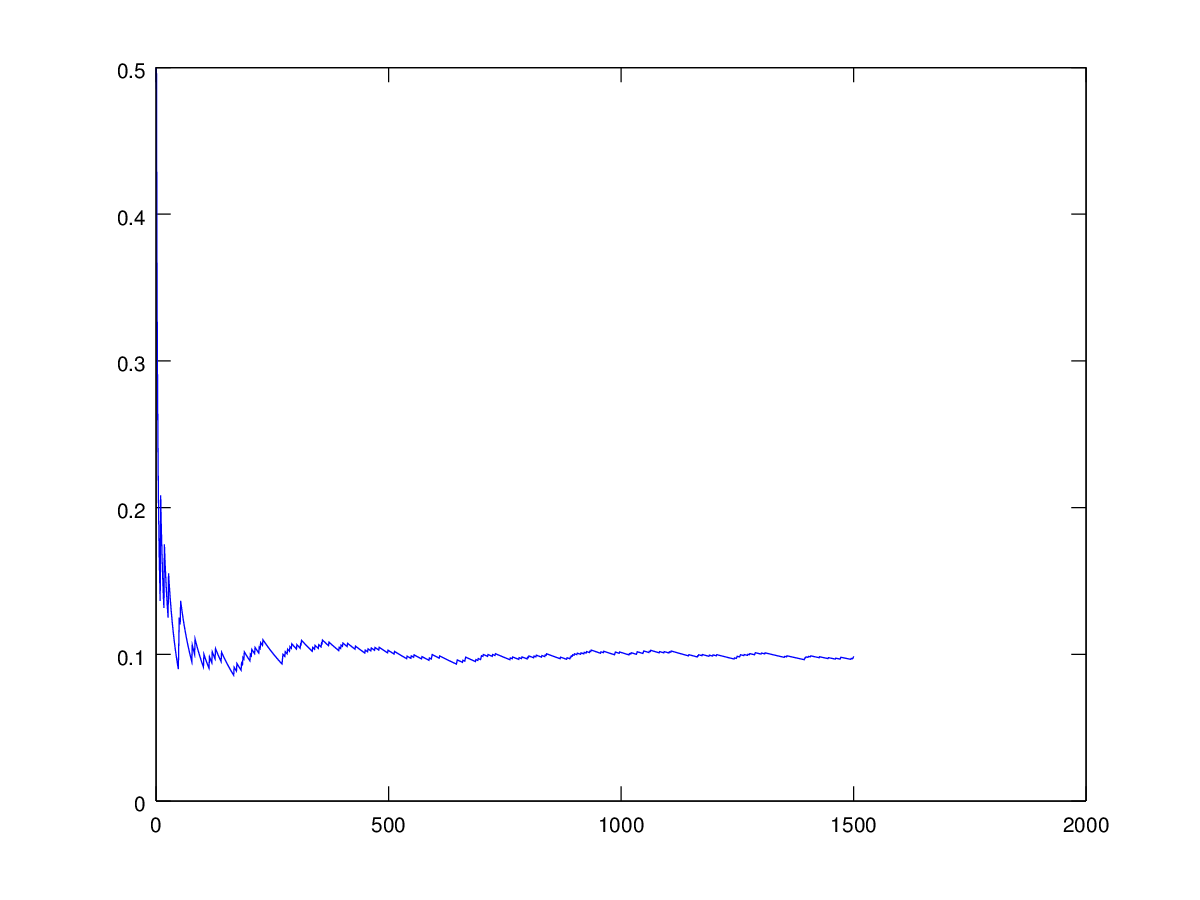
\includegraphics[width=10cm]{tarea2/poyla.PNG}}
\center{
	Gráfica de una ejecución de urnas de Poyla \\
	con 1 bola verde inicial, 1 bola roja inicial y constante 1.
}
\\


		\nqed
		
	\section{Tarea 3}

		\center{\includegraphics[width=10cm]{tarea3/poylaBeta.PNG}}
\center{
	Gráfica del histagrama de los radios \"finales\" de muchas iteraciones del proceso \\
	de urnas de Poyla.
}
\\

		\center{\includegraphics[width=10cm]{tarea3/galtonWatson.PNG}}
\center{
    Gráfica de una ejecución del proceso de extinción de Galton-Watson \\
    Parámetros: 10 individuos\\
    La probabilidad de que un individuo tenga $2$ hijos es $\frac{1}{2}$\\
        La probabilidad de que un individuo tenga $0$ hijos es $\frac{1}{2}$.
}
\\
	\bibliography{GenBib}
	\bibliographystyle{amsalpha}
\end{document}